\documentclass[lettersize,journal]{IEEEtran}
\usepackage{amsmath,amsfonts}
\usepackage{algorithmic}
\usepackage{algorithm}
\usepackage{array}
\usepackage[caption=false,font=normalsize,labelfont=sf,textfont=sf]{subfig}
\usepackage{textcomp}
\usepackage{stfloats}
\usepackage{url}
\usepackage{verbatim}
\usepackage{graphicx}
\usepackage{cite}
\usepackage{wasysym}
\usepackage{mathrsfs}



%
% \usepackage{biblatex}
%
% \usepackage[fleqn]{amsmath}
% \usepackage{amssymb}
% \usepackage{graphicx}
% \usepackage{cancel}
% \usepackage{tabularx}
%
% \usepackage{caption}
% % \usepackage{subcaption}
%
% \usepackage{subfig}
% \addbibresource{./citations.bib}
%
\graphicspath{ {C:/Users/Indy-Windows/Documents/MAE298_Intro_to_PDEs/images/} }

\newcommand{\volume}{{\ooalign{\hfil$V$\hfil\cr\kern0.08em--\hfil\cr}}}
%
% \usepackage{hyperref}
% \hypersetup{
% colorlinks=false,
% linkcolor=blue,
% filecolor=magenta,
%     urlcolor=blue,
% }
% \urlstyle{same}
% \setmathfont{XITS Math}
% updated with editorial comments 8/9/2021

\begin{document}

\title{MAE 298 Introduction to PDEs \\ Electrochemical Modeling of Batteries}

\author{Jonathan Dorsey}


% Remember, if you use this you must call \IEEEpubidadjcol in the second
% column for its text to clear the IEEEpubid mark.

\maketitle

% \begin{abstract}
% This
% \end{abstract}

\section{Introduction}
\IEEEPARstart{P}{artial} differential equations (PDEs) provide a mathematical basis for describing many significant scientific phenomena; however, while an important domain of study, in actually application it is often more challenging to understand and develop the PDE(s) that govern viable model than it is to understand the underlying mathematical formalism of PDEs. The inherent complexity of deriving and analyzing PDE models when compared to more approachable ODE models can be further exacerbated by coupled system of equations and/or nonlinear dynamics. For these systems, the derivation and interpretation of the model are often obfuscated by modeling assumptions, domain specific knowledge, and an understanding of how these mechanisms are translated into a PDE formation. In effect, these PDE models compromise higher model accuracy at the expense of ease of modeling, computational overhead, and intuition. An important modern day example can be found in the study of electrochemical battery modeling, where even simple electrochemical models of batteries consist of several coupled nonlinear partial differential equations. The objective of this paper is to derive the salient PDEs that describe a battery model known as the Doyle-Fuller-Newman (DFN) model, with enough context that the reader will be able to understand the development of the DFN model from the fundamental assumptions and mechanisms at play, and be able to understand how these concepts are translated into the language of Partial Differential Equations.

\section{Doyle-Fuller-Newman Model Overview}
The Doyle-Fuller-Newman model has long been held as the gold standard electrochemical battery model. This model describes at the first principle dynamics of a planar battery cell [Fig. \ref{DFN_schematic}]. This model encapsulates the dynamics of a lithium-ion battery at the continuum-scale. This is accomplished by derving the microscale governing equations and applying volume averages over the models' domain. The primary elements of this model consist of five governing equations for the conservation of mass in homogeneous solid phase, the conservation of charge in homogeneous solid phase, the conservation of mass in homogeneous electrolyte phase, the conservation of charge in the homogeneous electrolyte phase, and finally the transport effects of lithium movement between the solid and electrlye phases. The primary emphasis of this paper will be to investigate each category, and provide the context and first principles analysis which yield these governing PDEs. The governing equations for the microscale portion of the DFN model are shown below, the in order listed above.

\begin{figure}
  \centering
  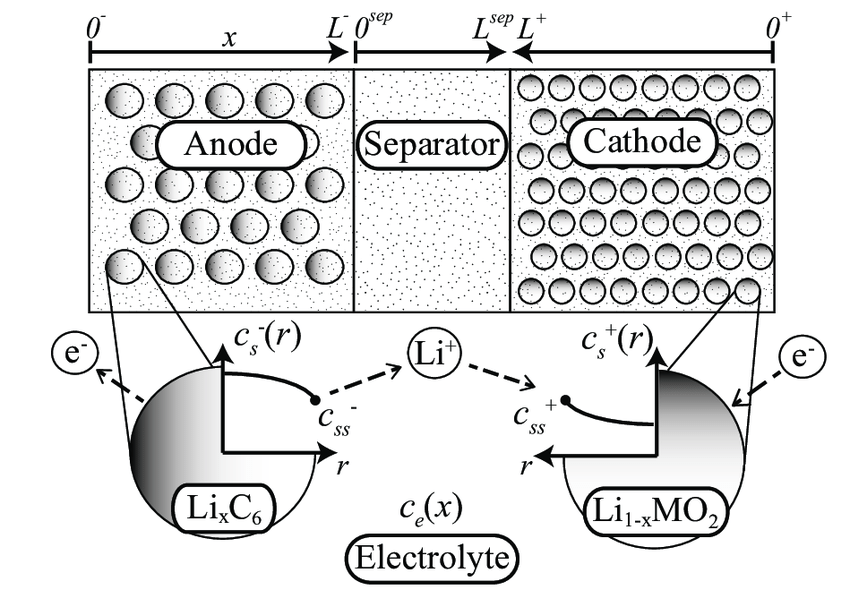
\includegraphics[scale=.25]{DFN}
  \caption{Planar DFN Model Schematic}
  \label{DFN_schematic}
\end{figure}

\begin{equation} \label{COC_s}
\nabla \cdot \mathbf{i}_{s}=\nabla \cdot\left(-\sigma \nabla \phi_{s}\right)=0
\end{equation}

\begin{equation} \label{COM_s}
\frac{\partial c_{s}}{\partial t}=\nabla \cdot\left(D_{s} \nabla c_{s}\right)
\end{equation}

\begin{equation} \label{COM_e}
\frac{\partial c_{e}}{\partial t}=\nabla \cdot\left(D_{e} \nabla c_{e}\right)-\frac{\mathbf{i}_{e} \cdot \nabla t_{+}^{0}}{F}-\nabla \cdot\left(c_{e} \mathbf{v}_{0}\right)
\end{equation}

\begin{equation}\label{COC_e}
\nabla \cdot \mathbf{i}_{e}=\nabla \cdot\left(-\kappa \nabla \phi_{e}-\frac{2 \kappa R T}{F}\left(1+\frac{\partial \ln f_{\pm}}{\partial \ln c_{e}}\right)\left(t_{+}^{0}-1\right) \nabla \ln c_{e}\right)=0
\end{equation}

\begin{equation} \label{lithium_movment}
j=\frac{i_{0}}{F}\left\{\exp \left(\frac{(1-\alpha) F}{R T} \eta\right)-\exp \left(-\frac{\alpha F}{R T} \eta\right)\right\}
\end{equation}

\section{Microscale Model Derivation}

As mentioned previously, Doyle-Fuller-Newman (DFN) model is a continuum-scale model; however, before this can be accomplished it is neccessary to compute the microscale dynamics of the battery. In the microscale model, the principle mechanisms of operation are evaluated under the assumption of homogeneous solid and electrolyte phases. Under this assumption, the model does not account for individual molecular interactions or impurities. This assumption implies that molecular inconsistencies will averaged out to create a homogeneous material that can be independently used to derive and evaluate the governing equations in both the solid and electroyte phases of the battery.

% The following sections will cover each of the primary governing equations for the microscale model in detail

\subsection{Charge Conservation in Homogeneous Solid}

From physics, it is know that charge must be conserved in an isolated system. For the purposes of this paper, we will assume that the battery we are modeling constitutes an isolated system that does not interact electrically with its environement. If the convseration of charge must hold, then it must be true that charge is not created or destroyed inside of the solid electrodes. This can be expressed as the following integral.

\begin{equation}
 I = - \iint_S \textbf{i} \cdot d \textbf{S}
\end{equation}

Where the net current into a volume \textbf{S} can be written in terms of the volume integral of the current density \textbf{i}. Via application of the Divergence Theorem and Conservation of Charge, it can be shown that ...

\begin{equation}
    I = - \iiint_{\volume} (\nabla \cdot \textbf{i})d{\volume} = 0
\end{equation}

Under these assumptions since the net currrent must be zero, the integrand must also be indentically equal to zero.

\begin{equation} \label{con_charg_solid}
    \nabla \cdot \textbf{i} = 0
\end{equation}

While this statement is an accurate formulation of the Conservation of Charge, we would like to formulate this same expressions as a function of electric potential, instead of current density. By applying the point form of \textbf{Ohm's Law}, namely $\textbf{i} = \sigma\textbf{E}$, where the electric field $\textbf{E} = -\nabla \phi$.

\begin{equation} \label{ohms_law}
  \textbf{i} = -\sigma \nabla \phi
\end{equation}

\noindent With this expression we can formulate the Convservation of Charge equation \#\ref{con_charg_solid}, as follows.

\begin{equation} \label{final_COC_s}
  \nabla \cdot (-\sigma \nabla \phi_s) = 0
\end{equation}


At anytime, equation \#\ref{final_COC_s}, must hold true in both electodes of the battery.

\subsection{Mass Conservation in Homogeneous Solid}

Next, the conservation of mass in homogeneous solid (electrodes) is used to capture the dynamics of lithium intercalation into the crystalline structure of the electrode materials. Specifically, this is a modeled by a diffusion process via Fick's first law, where the molar flux density \textbf{N} $[mol m^{-2} s^{-1}]$ is related to the gradient of lithium concentration in the solid electrode material, proportional to a material dependent constant of diffusivity D.
\begin{equation}\label{ficks_first}
    \textbf{N} =  -D \nabla c
\end{equation}

This expression states that the magnitude of the lithium molar flux density is proprotional to the gradient of the concentration; however, we would like to express it in terms of the time rate of change of the solid phase concentration. To accomplish this, we first need to compute the net molar flux by taking the integral of the net molar flux density over the entire domain boundary.
\begin{equation}\label{flux_divergence}
  j = -\oiint_{S} \textbf{N} \cdot \hat{\textbf{n}}dS
\end{equation}

This gives use the net molar flux \textbf{j} $ [mols_{-1}]$, which can rewritten in terms a molar flow rate, where n is the number of moles of lithium ...

\begin{equation}\label{molar_flux}
    j = \frac{dn}{dt}
\end{equation}

Recalling that the definition of molar concentration is the number of moles of a material over the total volume it occupies.

\begin{equation}
    n = \frac{c}{\volume}
\end{equation}

Given this definition, the number of moles $dn$ can be computed by integrating each contribution of concentration within a differential volume over the entire volume of the domain.
\begin{equation}
    n = \iiint_{\volume} cd{\volume}
\end{equation}

\noindent By taking the derivative with respect to time...
\begin{equation}\label{time_rate_of_molar_flux}
  \frac{dn}{dt} = -\frac{d}{dt} \iiint_{\volume} cd{\volume}
\end{equation}

\noindent By substituting equations \ref{molar_flux} and \ref{time_rate_of_molar_flux} into equation \ref{flux_divergence} we arrive at the following expression...
\begin{equation}\label{COM_s_int_form}
  \oiint_S \textbf{N} \cdot \hat{n}dS = -\frac{d}{dt} \iiint_{\volume} c d{\volume}
\end{equation}

This is the integral form of the continuity equation. This expression relates the molar flux density, which was in the original formulation of Fick's First Law in equation \ref{ficks_first}, to the concentration of lithium in the solid phase. This formulation is important because the concentration of lithium is a key component of developing the state of charge for electrochemical battery models. Additionally, as a continuity equation, it states that no mass has been created or destroyed inside the domain, further implying that all mass transfer happens only at the boundaries of the domain. Equation \ref{COM_s_int_form} can be further simplified into the more familiar point form of Fick's second law, as shown below.

\begin{equation}
    \frac{\partial c_{S}}{\partial t} = \nabla \cdot \left( D_{S} \nabla c_{s} \right)
\end{equation}

This law states that the total lithium flux density (in a given volume) must be equal to the rate of change of concentration within that volume.


\subsection{Charge Conservation in Homogeneous Electrolyte}

When discussing the conservation of charge inside of the electrolyte phase of the battery, a non-trivial amount of thermodynamics and physical chemistry are required to fully contextualize and provide the groundwork which needs to be laid, to understand the principles for deriving the governing equations. \\

This section will endeavour to lay the foundation for the elements of \textbf{Concentrated Solution Theory}, which are required to formulate the basic tenents of charge conservation in non-trivial chemical solutions, such as a batteries electrolyte.

\subsubsection{Gibbs Free Energy}
A simple definition of Gibbs Free Energy is total energy required to create the system (with internal energy u), plus the amount which boundary work (pV) required to make room for the system, minus the energy which is obtained from the surrounding environement (TS), which has a temperate of T. Conceptually, the Gibbs Free Energy is the amount of useful energy which can be harnessed to do work in the system.

\begin{equation} \label{gibbs_free_energy}
  G = U + p{\volume} - TS
\end{equation}

 The \textbf{free energy} portion of the name, is important because it informs us of how much energy can be extracted from the system, so long as the temperature and pressure are held constant. Additionally, the sign of the Gibbs free energy dictates the direction that a chemical reaction will spontaneously take. \\

 In the context of batteries, Gibbs free energy is used in the formulation of electrochemical potentials, which are discussed below.\\


 \subsubsection{Molarity \& Molality}

 Since an electrolyte is a solution, it can be described as an intensive property via its molarity and molality, depending on which attributes of the solution are of interest. The molarity of a solution is defined to be the number of moles of solute per liter of solution.

\begin{equation}\label{molarity}
    c_i = \frac{n_{solute_i}}{{\volume}_{solution}}
\end{equation}


 \noindent Where as the molality of the solution, is defined to be the total number of moles of solute over the mass of the solvent.

 \begin{equation}\label{molality}
     m_i = \frac{n_{solute_i}}{m_{solvent}}
 \end{equation}

 \subsubsection{Electrochemical Potential}

 Understanding the previous sections is important because it leads to a discussion of electrochemical potentials. Especially in multispecies solutions, the conversion from extensive properties to intensive properties is subtle. In order to properly define these intensive properties, it is neccessary to define partial molar quantities. This can be written using partial derivatives and describes how much the Gibbs free energy (extensive) changes with the addition of only species to the solution. This can be written...

 \begin{equation}\label{electrochemical_potential}
     \bar{\mu} = \left( \frac{\partial G}{\partial n_{i}} \right)_{T,p,n_{j} (j \neq i)}
 \end{equation}

 \noindent where $n_i$ is the number of moles of species $i$, while keeping the temperature, pressure, and moles of other species constant.  Given this definition, note that electrochemical potential is an intensive property which has been normalized via the species mass (in moles).\\

 As can be seen by substituting equation \ref{gibbs_free_energy} into equation \ref{electrochemical_potential}, the total potential is comprised of several components, including internal and external potentials. This distinction between internal and external potentials can be written as...

\begin{equation}
  \bar{\mu_{i}} = \bar{\mu}_{i, internal} + \bar{\mu}_{i, external}
\end{equation}

 In the absence of other potentials and forces from external fields, the effect of chemical and electrochemical potentials can be written as ...
 \begin{equation}\label{total_potential}
   \bar{\mu}_{i} = \mu_{i} + z_i F \phi
 \end{equation}

Where the $z_i$ is the charge number, $F$ is Faraday's constant, and $\phi$ is the local electrostatic potential.
This equation neatly seperates the potential contributions from both chemical and electrical mechanisms. After applying Euler's theorem for homogeneous functions we can show that.

\begin{equation}
  G(\textbf{n}) = \textbf{n} \cdot \nabla G (\textbf{n}) = \sum_i n_i \frac{\partial G}{\partial n_i}
\end{equation}

\begin{equation}\label{gibbs_summation}
  G = \sum_i n_i \bar{\mu}_i
\end{equation}

\noindent This provides a very concise form for relating the Gibbs free energy of our battery with the total potentials (chemical \& electrical) of the battery.  \\

\subsubsection{Gibbs-Duhem Equation}
The \textbf{Gibbs-Duhem} equation provides an important relationship between electrochemical potentials, which reduces the number of simultaneous equations which we must solve. It's derivation begins with the Gibbs Free Energy as shown below.

\begin{equation}
  G = U + pV - TS
\end{equation}

\begin{equation}
    dG = dU + d(pV) - d(TS)
\end{equation}

\begin{equation}
  = dq + dw + pdV + VdP -TdS - SdT
\end{equation}

\noindent Note that so far, all that has been accomplished has been applying a derivate and expanding the expression via the product rule of differentiation. From thermodynamics we know $dw = -pdV$ and that under the assumption of reversibility $dq = TdS$. After applying these substitutions, we arrive at the simplifed expressions below.

\begin{equation}
  dG = Vdp - SdT
\end{equation}

We can use equations \ref{electrochemical_potential} and \ref{gibbs_summation} to write the previous equation in terms of the total potential.
\begin{equation}
  \sum_{r}^{i=1} n_id\bar{\mu}_i = Vdp - SdT
\end{equation}

\noindent By rearranging the equations we get ...

\begin{equation}
  \sum_{i=1}^{r} n_id\bar{\mu}_i - Vdp + SdT = 0
\end{equation}

\noindent If we assume that pressure and temperature are constant, then derivatives of $p$ and $T$ are both zero. Since we expect to operate the battery in a constant temperature and pressure environment, these are meaningful simplifications which yield the following expression for a system with $i$ chemical species.

\begin{equation}
  \sum_{i=1}^{r} n_id\bar{\mu}_i = 0
\end{equation}

In the special case we are interested in (e.g a binary electrolyte) containing only two species, this equation can be explicitly written as

\begin{equation}\label{gibbs_duhem_eqn}
  n_1 d\bar{\mu}_1 + n_2 d\bar{\mu}_2 = 0
\end{equation}

This is an important equation because it directly governs the relationship between the two potentials. If one is increased, the other must decrease to maintain the equality. We can leverage this relationship to eliminate an equation, in future calculations, since we can write either quantity in terms of the other. This equation can also be written using the concentration of each species by dividing by the total volume.
\begin{equation}
  \sum_{i=1}^{r} c_{i}d\bar{\mu}_i = 0
\end{equation}

\subsubsection{Activity}

Unlike non-ionic solutions, ionic solutions do not distribute their ions randomly, this is because the electrical charge for either a cation or anion are preferentially oriented and attracted to ions of the opposite charge. A consequence of this behavior is that movement of ions in solution are artificially slow, due to the movement of a specific ion also attempting to drag the other ions which are in its immediate neighborhood in the solution. \\

Because of this phenomenon, we define \textbf{activity} of a species as an effective concentration, which accounts for this descrepency.

\begin{equation}\label{activity}
  a_i = c_i f_i
\end{equation}

In the context of lithium-ion batteries, the concept of activity is important because the transport medium between each electrode is a neutral ionic solution, which has a fixed number of positive and negative charge carries, that faciliate transfer of charge inside the battery. Therefore modeling this non-intutiative behavior is an important step in capturing the complete dynamics at play. \\

\subsubsection{ Stoichiometric Coefficient $\nu$ }
In a balanced chemical equation, the total amount of matter (of each element/molecule) and the total amount of charge are conserved. This fact holds true for electrolytes. In the case of an electrolyte, the solution is comprised of solute dispursed throughout a solvent such that the overall solution is charge-neutral. An example is shown below.

\begin{equation}
  \mathrm{Na}_{2} \mathrm{SO}_{4} \rightarrow 2 \mathrm{Na}^{+}+\mathrm{SO}_{4}^{2-}
\end{equation}

In this example, the coefficents in from of each ion on the right-hand-side of the equation, are known as \textbf{stoichiometric coefficients}, and are denoted with the symbol $\nu$. In the equation shown above, the stoichiometric coefficents are $\nu_{Na^{+}} = 2$ and $\nu_{SO_{4}^{2-}} = 1$.

\subsubsection{ Charge Number }

Similar to the stoichiometric coefficents, the \textbf{charge number} is also displayed in the chemical equation, as the super-script for each compound on the right-hand-side of the the balanced chemical equation. The charge number tells us how many excess electrons or protons exist in each given ion compound. The charge numbers for the equation above are $z_{Na^{+} = 1}$ and $ z_{SO_{4}^{2-}} = -2 $. The sign of the charge number informs us whether each compound is a cation ($z>0$) or anion ($z < 0 $)

\subsubsection{ Electroneutrality in Binary Electroytes }
As mentioned previously electroneutrality is an important and frequently referenced concept in the developement of the equations. In particular, a binary electrolyte comprised of only species is of particular interest and has useful properties which are very relavent to lithium-ion battery models. Under the constraint of charge-neutrality, we can state that the net charge in the solution must be $q = 0$. This can be expressed via charge numbers and the stoichiometric coefficents described above as follows.

\begin{equation}
  \sum_{i} z_{i} v_{i}=0
\end{equation}

For the general case the subscripts indicated whether the charge is from a cation or an anion, or the contributions form the solvent.

\begin{equation}
  z_{+} v_{+}+z_{-} v_{-}+z_{0} v_{0}=0
\end{equation}

However, since the solvents in the electroyte are always charge neutral, we can ommit them from this equation, leavinging the following expression.


\begin{equation}
  z_{+} v_{+}+z_{-} v_{-}=0
\end{equation}

\begin{equation}
  \frac{c_{+}}{v_{+}}=\frac{c_{-}}{v_{-}}
\end{equation}

This can be translate from stoichiometric coefficients to the ion concentration of each species, through the fact that we know these quanties are proportional to each other where the constant of proportionality is the concentation of the solution in general.

\begin{equation}
  c = \frac{c_{+}}{\nu_{+}} = \frac{c_{-}}{\nu_{-}}
\end{equation}

We can make use of this attribute and rewrite the charge neutrality equation as follows.


\begin{equation}
  \sum_{i} z_i c_i = 0
\end{equation}

Where $ i=2$ for our use-case of a binary electrolyte. This expression will be useful later when deriving the conservation of charge in an electrolyte.

\subsubsection{ Current Flow in Electrolyte }

Current flow inside of the electrolyte is comprised of both cations and anions. Therefore the total current flow inside of the electrolyte is given by

\begin{equation}
  i = i_{+} + i_{-}
\end{equation}

The next step is try write these ionic currents in terms of flux density so that they can be written in standard form later. This is accomplished by accounting for the amount of charge per second (for both cations and anions), due to the respective flux.

\begin{equation}
    i_+ =  z_+ FN_+ = z_{+}Fc_{+}v_{+}
\end{equation}

\begin{equation}
  i_- =  z_- FN_- = z_{-}Fc_{-}v_{-}
\end{equation}

Upon reflection of the quanities used in this expression we can see that the product of charge number, Faraday's constant, and flux density, is the eletrical current produced for the given charge type (positive/negative).


Therefore,

\begin{equation}
  i = z_{+}Fc_{+}v_{+} + z_- FN_- = z_{-}Fc_{-}v_{-}
\end{equation}

\begin{equation}
  = F\sum_{i}z_{i}N_{i}
\end{equation}

\subsubsection{ Deriving Conservation of Charge }

To begin this derivation, we can start off with the general expression for the conersation of mass at any point in a solution.

\begin{equation}
  \frac{\partial c_{i}}{\partial t}=-\nabla \cdot \mathbf{N}_{i}+R_{i}
\end{equation}

This version of Ficks Law states that the time rate of change on the concentration for species $i$ is related to the negative flux density gradient of that species as well as the rate of generation of species $i$.

\begin{equation}
  F \frac{\partial z_{i} c_{i}}{\partial t}=-\nabla \cdot\left(z_{i} F \mathbf{N}_{i}\right)+z_{i} F R_{i}
\end{equation}

Via algebra, we can multiply each side of the equation by $z_{i}F$ to get,

\begin{equation}
  \frac{\partial}{\partial t} F \sum_{i} z_{i} c_{i}=-\nabla \cdot\left(F \sum_{i} z_{i} \mathbf{N}_{i}\right)+F \sum_{i} z_{i} R_{i}
\end{equation}

Since the previous equation was written only with respect to a single species in the equation, we need to sum the same equation over each species resulting in the following...

\begin{equation}
  \frac{\partial}{\partial t} F \sum_{i} z_{i} c_{i}=-\nabla \cdot\left(F \sum_{i} z_{i} \mathbf{N}_{i}\right)
\end{equation}

As mentioned in the previous section about charge neutrality, we can see that our previous equation that the summation $\sum_{i}z_{i}c_{i}$ must be identically equation to zero since, the overall charge of the electrolyte is zero. We can also that the term $F\sum_{i}z_{i}N_{i}$ matches our previous definition for current shown above. By substituting these terms into the previous expression we arrive at the following equation.

\begin{equation}
  \nabla \cdot \mathbf{i}=0
\end{equation}

This equation is the differential form for the conservation of charge inside the electrolyte, stating that charge and not be created or destroyed.














\subsection{Mass Conservation in Homogeneous Electrolyte}



This next section is one of the most challenging to conceptualize as it has a great deal of nuance and complexity. \\

\subsubsection{Maxwell-Stefan Relationship}
This section lays the mathematical groundwork for the interaction of particles of differing species and the net force associated with these collisions. By applying the conservation of momentum, we can define the following expression for using average species velocities, for a 2 species mixture.

\begin{equation}
  m_{1} \mathbf{v}_{m_{1}}+m_{2} \mathbf{v}_{m_{2}}=m_{1} \mathbf{v}_{m_{1}}^{\prime}+m_{2} \mathbf{v}_{m_{2}}^{\prime}
\end{equation}

Given that the change in momentum for a single species can be written as...

\begin{equation}
  \Delta\left(m_{1} \mathbf{v}_{m_{1}}\right)=m_{1}\left(\mathbf{v}_{m_{1}}-\mathbf{v}_{m_{1}}^{\prime}\right)
\end{equation}

We can isolate the post-collision velocity of species 1, as follows.

\begin{equation}
  \mathbf{v}_{1}^{\prime}=\frac{m_{1} \mathbf{v}_{1}+m_{2} \mathbf{v}_{2}}{m_{1}+m_{2}}
\end{equation}

These two previous expressions can be combined to form the following equation.

\begin{equation}
  \begin{aligned}
  \Delta\left(m_{1} \mathbf{v}_{1}\right) &=m_{1}\left(\mathbf{v}_{1}-\mathbf{v}_{1}^{\prime}\right) \\
  &=m_{1}\left(\mathbf{v}_{1}-\frac{m_{1} \mathbf{v}_{1}+m_{2} \mathbf{v}_{2}}{m_{1}+m_{2}}\right)
  \end{aligned}
\end{equation}

Which can be simplified to...

\begin{equation}
  =\frac{m_{1} m_{2}}{m_{1}+m_{2}}\left(\mathbf{v}_{1}-\mathbf{v}_{2}\right)
\end{equation}

\subsubsection{Momentum Charnge Rate}
Now the task is to relate the change of momentum equation (on a mass basis) to the equivalent form on a species concentration basis. Generally speaking we can state that as the concentions of either species in a two species mixture increase the change in momentum should increase propotionally. Putting this intuition into math, we arrive at the following statement.

\begin{equation}
  \left(\frac{\mathrm{dp}}{\mathrm{d} t}\right)_{V}^{\text {species- }} \propto c_{1} c_{2}\left(\mathbf{v}_{1}-\mathbf{v}_{2}\right)
\end{equation}

From this statement, we can use the definition of the mole fractino $x_i = n_i /n$, where $n_i$ is the number of moles of a given species and $n$ is the total number of moles in the system. This defines the following relationship $x_1 + x_2 = 1$ for a binary species and in general form can be written as $\sum_i x_i = 1$. Furthermore, we can define a quantity called the total concentration, such that.

\begin{equation}
  C_{T}=\sum_{i} c_{i}
\end{equation}

Where concentration is defined as $c = n/ V$.  From this relationship we can show that.

\begin{equation}
  x_{i}=\frac{n_{i}}{n}=\frac{n_{i} / V}{n / V}=\frac{c_{i}}{c_{T}}
\end{equation}

Which can be substituted directly into the change of momentum equation to produce...

\begin{equation}
  \left(\frac{\mathrm{d} \mathrm{p}}{\mathrm{d} t}\right)_{V}^{\text {species- }} \propto x_{1} x_{2}\left(\mathrm{v}_{1}-\mathrm{v}_{2}\right)
\end{equation}

From undergraduate physics we know from Newton's Second law that force is equivalent to the time rate of change of momentum, leading us to the following statement.

\begin{equation}
  \mathrm{F}_{1, \mathrm{~V}} \propto x_{1} x_{2}\left(\mathrm{v}_{1}-\mathrm{v}_{2}\right)
\end{equation}

In order to turn this proportionality into an equality we must define a constant of proportionality. Given the current form of this statement relating force to a type of relative velocity, we could guess that this constant would behavior very closely to a coefficient of friction, $K_{ij}$. In addition to this, we would like to break down this parameter, since it in itself is not a constant number since its value depends on that mole fraction and hence the concentration of the species in the system.

\begin{equation}
  K_{i j} \propto x_{1}x_{2}
\end{equation}

It turns out that the resulting equality has been defined in terms of the Maxwell-Stefan diffusivity $mathscr{D}$, and the surrounding pressure.

\begin{equation}
  \mathscr{D}_{i j}=\frac{x_{i} x_{j}}{K_{i j}} p
\end{equation}

By applying the ideal gas law and substituting the concentration form of the mole fraction developed earlier, we get.

\begin{equation}
  K_{i j}=\frac{R T c_{i} c_{j}}{c_{T} \mathscr{D}_{i j}}
\end{equation}

After developing these expressions, we can subsitute them back into the original equation for the force acting on species 1.

\begin{equation}
  \mathbf{F}_{1, V}=\frac{R T c_{1} c_{2}}{c_{T} \mathscr{D}_{12}}\left(\mathbf{v}_{1}-\mathbf{v}_{2}\right)
\end{equation}

Now that we have an expression for the force acting on a species , we can begin to make the connections between forces and the electrochemical potential for charged species. \\


\subsubsection{Multicomponet Diffusion Equation}

We know that we can write force as the negative gradient of a potential function. In our case, this potential function is the Gibbs free energy developed previously.

\begin{equation}
  \mathrm{F}_{1}=-\nabla G_{1}=-\frac{\partial G_{1}}{\partial \mu_{1}} \nabla \bar{\mu}_{1}=-n_{1} \nabla \bar{\mu}_{1}
\end{equation}

By equating this equation with the expression for force developed above, we get the following equation.

\begin{equation}
  c_{1} \nabla \mu_{1}=R T \frac{c_{1} c_{2}}{c_{T} \mathscr{D}_{12}}\left(\mathbf{v}_{2}-\mathbf{v}_{1}\right)
\end{equation}

This can be re-written...

\begin{equation}
  c_{i} \nabla \mu_{i}=R T \sum_{j} \frac{c_{i} c_{j}}{c_{T} \mathscr{D}_{i j}}\left(\mathbf{v}_{j}-\mathbf{v}_{i}\right)=\sum_{j} K_{i j}\left(\mathbf{v}_{j}-\mathbf{v}_{i}\right)
\end{equation}

After summing over all species in the mixture.

\begin{equation}
  \sum_{i} c_{i} \nabla \mu_{i}=\sum_{i} \sum_{j} K_{i j}\left(\mathbf{v}_{j}-\mathbf{v}_{i}\right)
\end{equation}

\subsubsection{Concentrated Binary Electrolyte Theory: Ion Fluxes}

\begin{equation}
  \mathrm{F}_{1, V}=\frac{\mathrm{F}_{1}}{V}=-\frac{n_{1}}{V} \nabla \mu_{1}=-c_{1} \nabla \beta_{1}
\end{equation}

\begin{equation}
  \frac{\partial c}{\partial t}=\nabla \cdot\left[D\left(1-\frac{\mathrm{d} \ln c_{0}}{\mathrm{~d} \ln c}\right) \nabla c\right]-\frac{\mathbf{i} \cdot \nabla t_{+}^{0}}{z_{+} v_{+} F}-\nabla \cdot\left(c \mathbf{v}_{0}\right)
\end{equation}


\subsection{Lithium Movement Between Solid \& Electrolyte Phases}


\section{DFN Model Derivation}

The previous system of governing partial differential equations, was derived using the microscale interactions and mechanisms. While this approach to analysis is particularly informative about the how these sorts of high fidelity models are derived, solving them for an entire cell (using a system of thousands or millions of coupled PDEs) is computationally infeasible, even for modern computers. There are many different approaches to creating macroscale models that capture the first principle mechanisms of action, but are far more computationally viable. This simplification comes with a penalty on the accuracy of model; however, these models are still far and away some of the most high fidelity battery models which are routinely used today to check  \\

In particular, the Doyle-Fuller-Newman (DFN) model uses a technique of volume averaging to be able to same governing equations which were derived above, over larger domains, approximating (on average) the behaviors of each electrode and the electrolyte. \\

\subsection{Volume Averaging Methods}

blah blah blah

\section{Single Particle Model (SPM \& SPMe)}

As mentioned previously the microscale and macroscale models described above are computationally very expensive to compute numerical solutions for. Due to this property, these models are often not used as a practical work-horse models for the daily needs of systems that incorporate battery models, and that model like the DFN formulation, are generally used as benchmarks of accuracy and performance for a reduced-order or BLANK battery models. These simplified models usually sacrifice a great deal of the accuracy which the DFN model worked so hard to preserve from first principles. As a consequence, model such as a simple lookup-table or equivalent circuit model (ECM) are dominately purposed around the use of real-time systems that need a roughly accurcate computation about the state of charge of a cell. However, there are use-cases where these simplified models are too low resolution, and require higher fidelity models, that are slightly more expensive to compute, but provide much better tracking to the DFN base-line model. \\

Two such model variations are the Single Particle Model (SPM) and the Single Particle Model with Electrolyte Dyanmics (SPMe). These models are far an away the work-horse of many battery control and estimation tasks. The guiding principle of these models is to focus on the dominate dynamics of the battery. It is a well known fact presented in undergraduate control theory that the slowest pole/zero will dominate the transient dynamics for a given linear system. For lithium ion batteries, it can be shown that the diffusion of lithium into the solid-phase (electode) evolves ths slowest, and therefore dominates the dynamic behavior of the battery for the time-scales which we are mostly interested in. The SPM model takes this fact and reduces each electrode, of the battery, to an individual sphere of active material that is presumed to be representative of the average dynamics of the electrodes. It should be notes that in this model, another simplification is made whereby the electolyte concentration and dynamics are discarded. The SPMe elevates the SPM model by including these electrolyte dynamics back into the model, allowing this model to capture the nonlinearities which are present due to transport behavior of the electrolyte.



\section{Analysis of Governing Equations}

\section{Numerical Solution}

\section{Results}

\section{Conclusion}
The conclusion goes here.


\section*{Acknowledgments}
This should be a simple paragraph before the References to thank those individuals and institutions who have supported your work on this article.

\section{References Section}
You can use a bibliography generated by BibTeX as a .bbl file.
 BibTeX documentation can be easily obtained at:
 http://mirror.ctan.org/biblio/bibtex/contrib/doc/
 The IEEEtran BibTeX style support page is:
 http://www.michaelshell.org/tex/ieeetran/bibtex/

 % argument is your BibTeX string definitions and bibliography database(s)
%\bibliography{IEEEabrv,../bib/paper}
%
\section{Simple References}
You can manually copy in the resultant .bbl file and set second argument of $\backslash${\tt{begin}} to the number of references
 (used to reserve space for the reference number labels box).

\begin{thebibliography}{1}
\bibliographystyle{IEEEtran}

\bibitem{ref1}
{\it{Mathematics Into Type}}. American Mathematical Society. [Online]. Available: https://www.ams.org/arc/styleguide/mit-2.pdf

\bibitem{ref2}
T. W. Chaundy, P. R. Barrett and C. Batey, {\it{The Printing of Mathematics}}. London, U.K., Oxford Univ. Press, 1954.

\bibitem{ref3}
F. Mittelbach and M. Goossens, {\it{The \LaTeX Companion}}, 2nd ed. Boston, MA, USA: Pearson, 2004.

\end{thebibliography}


\newpage

\section{Biography Section}

\vspace{11pt}

% \bf{If you include a photo:}\vspace{-33pt}
% \begin{IEEEbiography}[{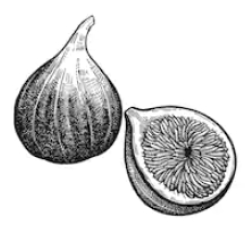
\includegraphics[width=1in,height=1.25in,clip,keepaspectratio]{fig1}}]{Michael Shell}
% Use $\backslash${\tt{begin\{IEEEbiography\}}} and then for the 1st argument use $\backslash${\tt{includegraphics}} to declare and link the author photo.
% Use the author name as the 3rd argument followed by the biography text.
% \end{IEEEbiography}

\vspace{11pt}

\vfill

\end{document}
